% \documentclass[a4paper]{siamart220329}
\documentclass[a4paper]{siamonline220329} 
\usepackage{damacros}
\usepackage{amssymb}
\usepackage{bbm}
\usepackage{wrapfig}

% Theorem environment for questions: Small-caps header, italize body.
\theoremstyle{plain}
% \theoremheaderfont{\normalfont\sc}
\theoremheaderfont{\normalfont\bf} \theorembodyfont{\normalfont} \theoremseparator{.}
\theoremsymbol{} \newtheorem{question}{Question}
\renewcommand\phi\varphi

\crefname{question}{question}{questions}
\Crefname{question}{question}{questions}
 
\usepackage{listings}
\definecolor{LightGrey}{rgb}{0.9629411,0.9629411,0.9629411}
\definecolor{LighterGrey}{gray}{0.99}
\definecolor{Mauve}{rgb}{0.58,0,0.82}
\definecolor{Emerald}{rgb}{0.31, 0.78, 0.47}
\definecolor{RoyalBlue}{rgb}{0.25, 0.41, 0.88}
\definecolor{myGreen}{cmyk}{0.82,0.11,1,0.25}
\lstset{
    language=Matlab,
    keywordstyle=\color{RoyalBlue},
    basicstyle=\ttfamily,
    %commentstyle=\color{Emerald}\scriptsize\ttfamily,
    morekeywords={define,ifndef,endif},
    commentstyle=\color{myGreen}\scriptsize\ttfamily,
    %directivestyle=\color{Mauve}\scriptsize\ttfamily,
    showspaces=false,            
    showstringspaces=false,
    stringstyle=\color{Mauve}\scriptsize\ttfamily,
    numbers=left,
    numberstyle=\scriptsize,
    stepnumber=1,
    numbersep=8pt,
    showstringspaces=false,
    breaklines=true,
    frameround=ftff,
    frame=lines,
    backgroundcolor=\color{LightGrey}
} 

% Sets running headers as well as PDF title and authors
\headers{Finite-Element simulation of neural fields}{D. Avitabile}

% Title. If the supplement option is on, then "Supplementary Material" is
% automatically inserted before the title.
\title{Tutorial on Finite-Element schemes for neural fields} 

% Authors: full names plus addresses.
\author{ Daniele Avitabile
\thanks{ Vrije Universiteit Amsterdam, Department of
  Mathematics, Faculteit der Exacte Wetenschappen, De Boelelaan 1082a, 1082 HV
  Amsterdam, The Netherlands. \protect MathNeuro Team, Inria branch of the University
  of Montpellier, 861 rue Saint-Priest 34096 Montpellier Cedex 5 France. \protect
(\email{d.avitabile@vu.nl}, \url{www.danieleavitabile.com}). }
% \and Paul T. Frank \thanks{Department of Applied Mathematics, Fictional University,
% Boise, ID (\email{ptfrank@fictional.edu}, \email{jesmith@fictional.edu}).} \and
% Jane E. Smith\footnotemark[4]
}

\graphicspath{{./Figures/}}

\begin{document}

\maketitle

\begin{abstract}
  In this tutorial we study the implementation of a basic Finite Element method for a
  neural field equation with one or more components. We will also compute and
  visualise patterns of cortical activity supported by these models, and observed in
  experiments. Before starting this tutorial download the latest version of
  \href{https://zenodo.org/records/11120604}{the accompanying
  dataset}. Solutions to the exercises can be found here:
  \href{http://htmlpreview.github.io/?https://github.com/danieleavitabile/numerical-analysis-mathematical-neuroscience/blob/main/Tutorials/Tutorial2/Solutions/Question1/html/driver.html}{Q1},
  \href{http://htmlpreview.github.io/?https://github.com/danieleavitabile/numerical-analysis-mathematical-neuroscience/blob/main/Tutorials/Tutorial2/Solutions/Question2/html/driver.html}{Q2},
  \href{http://htmlpreview.github.io/?https://github.com/danieleavitabile/numerical-analysis-mathematical-neuroscience/blob/main/Tutorials/Tutorial2/Solutions/Question3/html/driver.html}{Q3},
  \href{http://htmlpreview.github.io/?https://github.com/danieleavitabile/numerical-analysis-mathematical-neuroscience/blob/main/Tutorials/Tutorial2/Solutions/Question4/Disk/html/driver.html}{Q4 (Disk)},
  and
  \href{http://htmlpreview.github.io/?https://github.com/danieleavitabile/numerical-analysis-mathematical-neuroscience/blob/main/Tutorials/Tutorial2/Solutions/Question4/Hexagon/html/driver.html}{Q4 (Hexagon)}.
  Code can be downloaded from
  \href{https://github.com/danieleavitabile/numerical-analysis-mathematical-neuroscience/tree/main}{our
  repository}.
\end{abstract}


\section{Introduction}\label{sec:introduction} 
This tutorial deals with the implementation of a basic Finite Element Scheme for the
standard Neural Field Equation
\[
  \label{eq:NF}
  \begin{aligned}
    \partial_{t} u(r,t) & = -u(r,t) + \int_{D} w(r,r') f(u(r',t))\,d r',
                        && (r,t) \in D \times [0,T] \\
    u(r,0) & = \phi(r)
           && r \in D.
  \end{aligned}
\]
posed on a generic cortical surface $D \subset \RSet^3$. The exposition is
non-technical, and downloadable exemplary files for relevant matrices are given to
simplify the tutorial at a first pass. At the end of the tutorial you will have
visualised patterns observed in experimental recordings of neuronal activity. A
theory for numerical schemes for neural fields is given in
\cite{avitabileProjectionMethodsNeural2023} (see also references therein).

\subsection{Domain and triangulation} \label{ssec:triangulation}

\begin{wrapfigure}{r}{0.5\textwidth}
  \begin{center}
    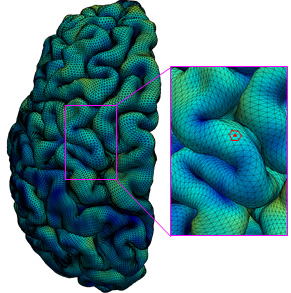
\includegraphics[width=0.4\textwidth]{brain-mesh}
  \end{center}
  \caption{Example of a cortical mesh
    \href{https://www.med.unc.edu/bric/scientists-create-new-map-of-the-developing-cerebral-cortex/}{(website)}
  }
\end{wrapfigure}
We will assume that the cortex $D$ to be a piecewise-smooth compact surface
$\RSet^3$. More specifically, $D$ is triangulated using $m$ triangles: we consider a
triangulation of $\calT = \{ \tau_\alpha \}_{\alpha = 1}^m$ of $D$ such
that 
\[ 
  \bigcup_{\alpha=1}^m \tau_\alpha = D, \qquad 
  \tau_\alpha^\circ \cap \tau_\beta^\circ = \varnothing, \quad \alpha \neq \beta 
\] 
where $\tau_\alpha^\circ$ denotes the interior of triangle $\tau_{\alpha}$. We will
denote by $\mu_\alpha$ the area of the triangle $\tau_\alpha$. We will use
$r=(x,y,z)$ for points in $\RSet^3$, and we number the nodes of the triangulation
from $1$ to $n$, with coordinates $\{ r_i \}_{i=1}^n$.


\begin{figure}
  \centering
  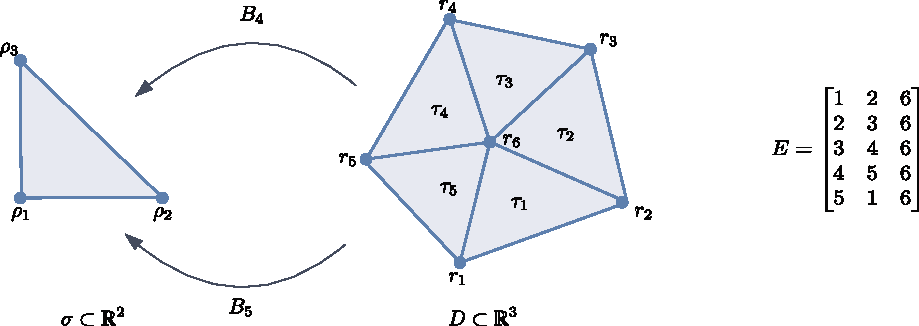
\includegraphics[width = 0.8\textwidth]{triangulation}
  \caption{A triangulation with $5$ elements for a domain $D \subset \RSet^3$. Each
  triangle is mapped to the standard simplex $\sigma \subset \RSet^2$. To the right
we show the corresponding element matrix $E$.}
  \label{fig:triangulation}
\end{figure}

It is convenient to introduce a family of mappings $\{ B_\alpha \}_{\alpha}$ which
send the reference triangle $\sigma$ (the standard simplex in $\RSet^2$) to the
triangles $\{\tau_\alpha\}_{\alpha}$, that is, $B_\alpha \colon \sigma \mapsto \tau_{\alpha}$.
The standard simplex in $\RSet^2$ is the triangle with nodes $\rho_1=(0,0)$,
$\rho_2=(1,0)$, $\rho_3=(0,1)$ (see schematic in \cref{fig:triangulation}).

In this tutorial we use matrices to encode information about triangulation.
Coordinates of the nodes are stored in a $n$-by-$3$ matrix $N$, so
that the $i$th row of $N$ contains the coordinates $r_i$, while triangular elements
are stored in an $m$-by-$3$ matrix $E$, so that the $\alpha$th row of $M$ indicates
that triangle $\tau_\alpha$ has vertices at nodes $\{ n_{\alpha,1},
  n_{\alpha,2}, n_{\alpha,3}\}$,
\[
  N =
  \begin{bmatrix} 
    x_1 & y_1 & z_1 \\
    x_2 & y_2 & z_2 \\
    \vdots & \vdots & \vdots \\
    x_n & y_n & z_n
  \end{bmatrix}, 
  \qquad 
  E =
  \begin{bmatrix} 
    n_{1,1} & n_{1,2} & n_{1,3}\\
    n_{2,1} & n_{2,2} & n_{2,3}\\
    \vdots & \vdots & \vdots \\
    n_{3,1} & n_{3,2} & n_{3,3}
  \end{bmatrix}.
\]

\subsection{Quadrature}\label{ssec:quadrature} We address the problem of
approximating the integral of a function $u \colon D \to \RSet$ over $D$. The
starting point is defining a quadrature rule over the simplex $\sigma$, for a
function $g \colon \sigma \to \RSet$. Rather than aiming for a general treatment,
we work with a concrete quadrature choice to simplify the notation (more
sophisticated quadrature rules can be obtained with minimal changes): its quadrature
nodes coincide with the vertices $\{ \rho_k \}_{k=1}^3$ of the simplex,
and its quadrature weights are equal to $1/6$ for each node, hence
\[
  \int_{\sigma} g(\rho) \,d \rho \approx
  \sum_{k=1}^3 g(\rho_k)/6, 
\]

Starting from this quadrature, we now write
\[
  \begin{aligned}
  \int_{D} u(r) \,d r'
  &
  = \sum_{\alpha=1}^m \int_{\tau_\alpha} u(r) \,d r 
  % \\
  % &
  = \sum_{\alpha=1}^m \int_{B_\alpha(\sigma)} u(r) \,dr
  % \\
  % &
  = \sum_{\alpha=1}^m \mu_\alpha \int_{\sigma} u(B_\alpha(\rho)) \,d\rho
  \\
  &
  \approx
  \sum_{\alpha=1}^m \mu_\alpha/6 \sum_{k=1}^3 u(B_\alpha(\rho_k)).
   \\
  \end{aligned}
\]

With a further manipulation of the terms in the latest sum, we can write the quadrature
formula above as a weighted sum of $u$ at the nodes of the triangulation 
\[
  \begin{aligned}
  \int_{D} u(r) \,d r
  &
  \approx
  \sum_{\alpha=1}^m \mu_\alpha/6 \sum_{k=1}^3 u(B_\alpha(\rho_k))
   % \\
  % &
  =
  \sum_{j=1}^{n} u(r_j) \sum_{\{ \alpha \colon r_j \in \tau_\alpha \}}
  \mu_\alpha/6
   \\
  &
  =:
  \sum_{j=1}^{n} u(r_j) \delta_j
   \\
  \end{aligned}
\]

Equipped with the quadrature rule of the previous section, we can now approximate the
integral of functions in the form $r' \mapsto w(r,r') v(r')$ 
\begin{equation}\label{eq:quadW}
  \int_{D} w(r,r') v(r')\,dr' \approx \sum_{j=1}^n w(r,r_j) v(r_j) \delta_j
\end{equation}

\subsection{Finite Element Collocation Scheme for Neural Fields}\label{ssec:scheme} 
We are now ready to formulate a finite element collocation scheme for \cref{eq:NF}.
We collocate \cref{eq:NF} at the nodes $\{ r_i \}_{i=1}^n$
\[
  \begin{aligned}
    \partial_{t} u(r_i,t) & = -u(r_i,t) + \int_{D} w(r_i,r') f(u(r',t))\,d r',
                        && i=1,\ldots,n, \quad t \in [0,T] \\
    u(r_i,0) & = \phi(r_i)
                        && i=1,\ldots,n,
  \end{aligned}
\]
and apply the quadrature rule \cref{eq:quadW} to arrive at the set of approximating ODEs
\begin{equation}\label{eq:ODE}
  U'(t) = -U(t) + MF(U(t)), \qquad t \in [0,T], \qquad U(0) = \Phi,
\end{equation}
where $U(t) \in \RSet^n$ for all $t \in [0,T]$ is a vector with components $U_i(t)
\approx u(r_i,t)$, the vector $\Phi \in \RSet^n$ has components $\Phi_i = \varphi(r_i)$, and the
nonlinear function $F \colon \RSet^n \to \RSet^n$, has components $(F(U))_i = f(u_i)$.
Finally the matrix $M \in \RSet^{n \times n}$ has components $M_{ij} =
w(r_i,r_j)\delta_j$.

\section{Tutorial questions}\label{sec:question} 

\begin{question}
  This question is to make you familiar with triangulation, meshes and plotting
  with their data structure. We aim to plot the function
  \[
    u(\rho,\theta) = a e^{-b \rho}(b\cos \rho  + \sin \rho ) \cos(\omega \theta),
    \qquad (r,\theta) \in [0,R] \times [-\pi,\pi)
  \]
  with parameters $a =10$, $b = 0.05$, $\omega =4$, $R = 30$. 

  In principle this task involves creating a triangulation of the disk of radius $R$,
  which is a nontrivial task. I suggest to skip this step at a first pass, and
  load a precomputed dataset, providing nodes and elements in matrices $N$ and
  $E$, respectively, in the format specified in \cref{ssec:triangulation}.

  \begin{enumerate}
    \item Download \href{https://zenodo.org/records/11120604}{the accompanying
  dataset}. The relevant data is in the folder \lstinline|Spots-Disk| folder
      in a binary file \texttt{mesh.mat}, which contains \texttt{nodes} and \texttt{elements} fields.
      This binary MATLAB format can be downloaded also in Python (see instructions
      \href{https://docs.scipy.org/doc/scipy/reference/generated/scipy.io.loadmat.html}{here}).
      Alternatively, the matrices $N$ and $E$ can be imported from the text files
      \texttt{nodes.dat} and \texttt{elements.dat}, respectively.
    \item Create a vector \texttt{u} whose $i$th components evaluates $u$ at the
      $i$th node, and plot the function. In Matlab, this can be done with a command
      along these lines
      \begin{lstlisting}[numbers=none]
trisurf(elements,x,y,z,u);
      \end{lstlisting}
      Plotting on triangulated meshes may not be straightforward, and you need to
      know how to do it for the remainder of the tutorial, so I have added a
      \lstinline|minimal-plotter.m| and \lstinline|minimal-plotter.py| to get you
      going. 
  \end{enumerate}
\end{question}

\begin{question}\label{question:kernels}
  Next, we create the Finite Element (FE) matrix $M$ appearing in \cref{eq:ODE}, for
  the following kernel
  \[
    w(r,r') = W_{A,\eps}(\| r - r' \|_2), 
    \quad 
    W_{A,\eps}(x) = 
    \begin{cases}
      A(x) & \text{if $|A(x)|  \geq \eps $,} \\
      0    & \text{otherwise,} 
    \end{cases},
    \quad 
    A(x) = e^{-bx}(b \sin x + \cos x )
  \]
  with parameters $b =0.4$, $\eps = 10^{-3}$.
  The synaptic kernel is thus distance dependent and truncated, meaning that only
  synaptic connections of sufficiently large strength are retained.

  One way to form $M$ (there are faster and cheaper ones) is to first create a matrix
  $W$ with components $W_{ij} =  w(r_i,r_j)$ and then assemble the FE matrix $M$ with
  components $M_{ij}=W_{ij}
  \delta_j$. The matrices $M$ and $W$ are sparse, and can be stored cheaply in sparse
  format, that is: one can store them cheaply specifying the matrix size, and three
  vector variables \lstinline|rows|, \lstinline|cols|, and \lstinline|vals|,
  containing rows, column and values of the nonzero entries of the matrix. In this
  way the $i$th nonzero entry of the
  matrix $M$ is specified as
      \begin{lstlisting}[numbers=none]
M(rows(i),cols(i)) = vals(i);
      \end{lstlisting}
  Working with sparse matrices also ensures that matrix-vector multiplications are
  carried out parsimoniously: if a matrix entry is null, we don't waste time using it
  in the multiplications. This results in large savings when one repeatedly evaluates
  the right-hand side of \cref{eq:ODE}. To get further information on sparse matrices,
  you could look into Matlab's  \lstinline|sparse| command
  (\href{https://nl.mathworks.com/help/matlab/ref/sparse.html}{here}), or SciPy's
  \lstinline|scipi.sparse|
  command (\href{https://docs.scipy.org/doc/scipy/reference/sparse.html}{here}).

  As for the previous question, you could write your own code to generate $M$, but I
  suggest to load the matrices $W$ and $M$ at a first pass. You can load
  $W$ and $M$ using the binary files \lstinline|synaptic-matrix.mat| and
  \lstinline|fem-matrix.mat|, or their corresponding text (\lstinline|.dat|) files.

  Write code that loads (or computes) the matrices $W$, and $M$. Visualise the
  sparsity pattern of the matrix $M$ (commands \lstinline|spy| in both Matlab and
  Python), and plot the function $r \mapsto W(r,r_{2000})$, the synaptic connections
  emanating from point $r_{2000}$ in the cortex.
\end{question}

\begin{question}\label{question:spots}
  Cortical regions can support patterns that occupy the full space, 
  (as we have seen in a previous tutorial on Turing-like bifurcations), as well as
  \textit{localised patterns of activity}. Spots of activity in brain experiments can
  be found in connection with grid cells \cite{haftingMicrostructureSpatialMap2005} (see
  also \href{https://www.youtube.com/watch?v=i9GiLBXWAHI}{this video}).

  In a localised pattern, high activity is found only in a confined region of the
  cortex, that remains inactive elsewhere. We are going to explore these patterns as
  solutions to the following neural field equation
\begin{equation}
  \begin{aligned}
    \partial_{t} u(r,t) & = -u(r,t) + \int_{D} w(r,r') f(u(r',t))\,d r',
      && (r,t) \in D \times [0,T] \\
    u(r,0) & = \varphi(r)
      && r \in D.
  \end{aligned}
\end{equation}
  The cortex $D$ is the disk of radius $R=30$, and the time horizon is fixed to
  $T=50$. The synaptic kernel is the one given in \cref{question:kernels}, with
  parameters $b =0.4$, $\eps = 10^{-3}$. The firing rate is given by
  \[
    f(u) = \frac{1}{1+e^{-\mu u+\theta}} - \frac{1}{1+e^{\theta}},
    \qquad \mu =5.5, \qquad \theta = 5.6,
  \]
  and the initial condition by 
  \[
    \varphi(r) = \frac{\alpha}{\bigl[\cosh(\beta \| r \|_2)\bigr]^2},
   \qquad \alpha = 20, \qquad \beta = \frac{1}{20}. 
  \]

  Run a simulation and produce numerical evidence that, when the system reaches an
  equilibrium, spots of activity form in a large portion of the cortex. This system
  is capable of sustaining many different configurations, in which spots are
  localised or not, and displaced in several parts  of the cortex.

  Perturb the system by setting $\mu =6$ and taking
  \[
    \phi(r) = 
    \begin{cases}
      u(r,T) & \text{if $\| r \|_2  \leq 15$,} \\
      0      & \text{otherwise,} 
    \end{cases}
  \]
  where $u(r,T)$ is the final state of the previous simulation. This perturbation
  changes the steepness of the sigmoid, and cuts the outer spots of the
  equilibrium found for $\mu = 5.5$. How does the system respond to this perturbation?
\end{question}

\begin{figure}
  \centering
  % 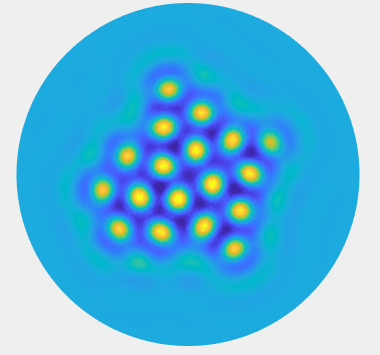
\includegraphics[width = 0.4\textwidth]{spots}
  % 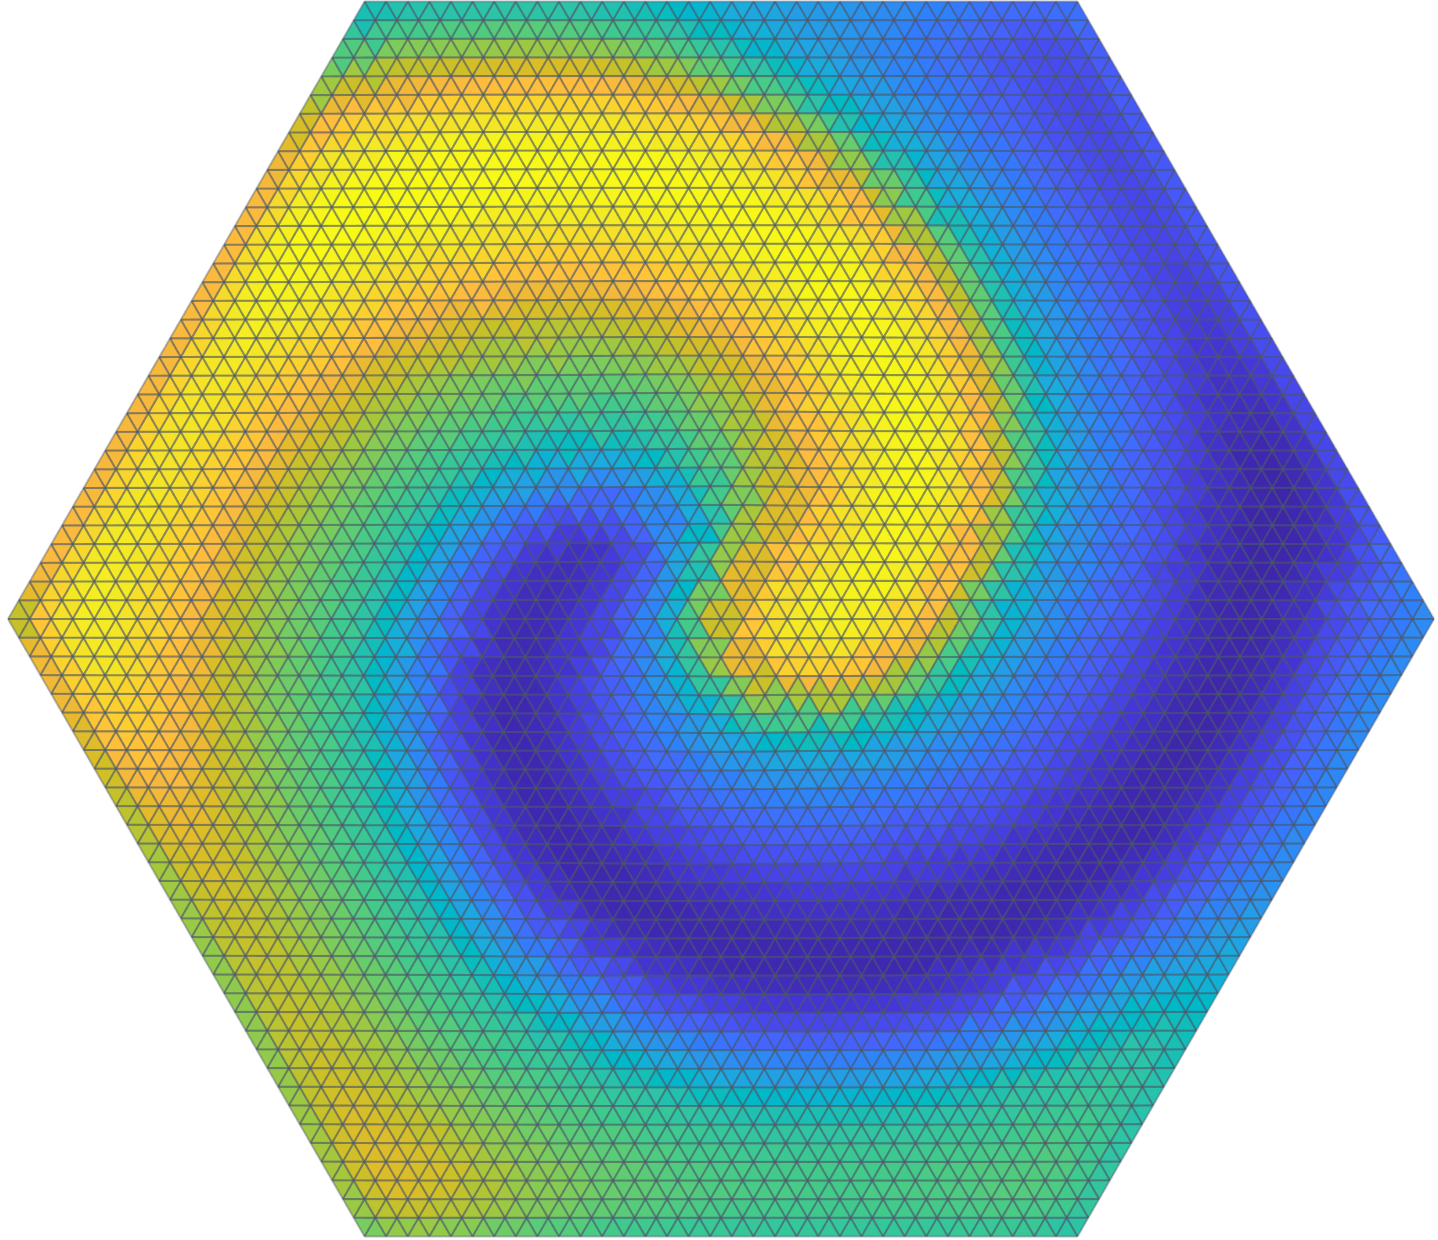
\includegraphics[width = 0.4\textwidth]{spiral}
  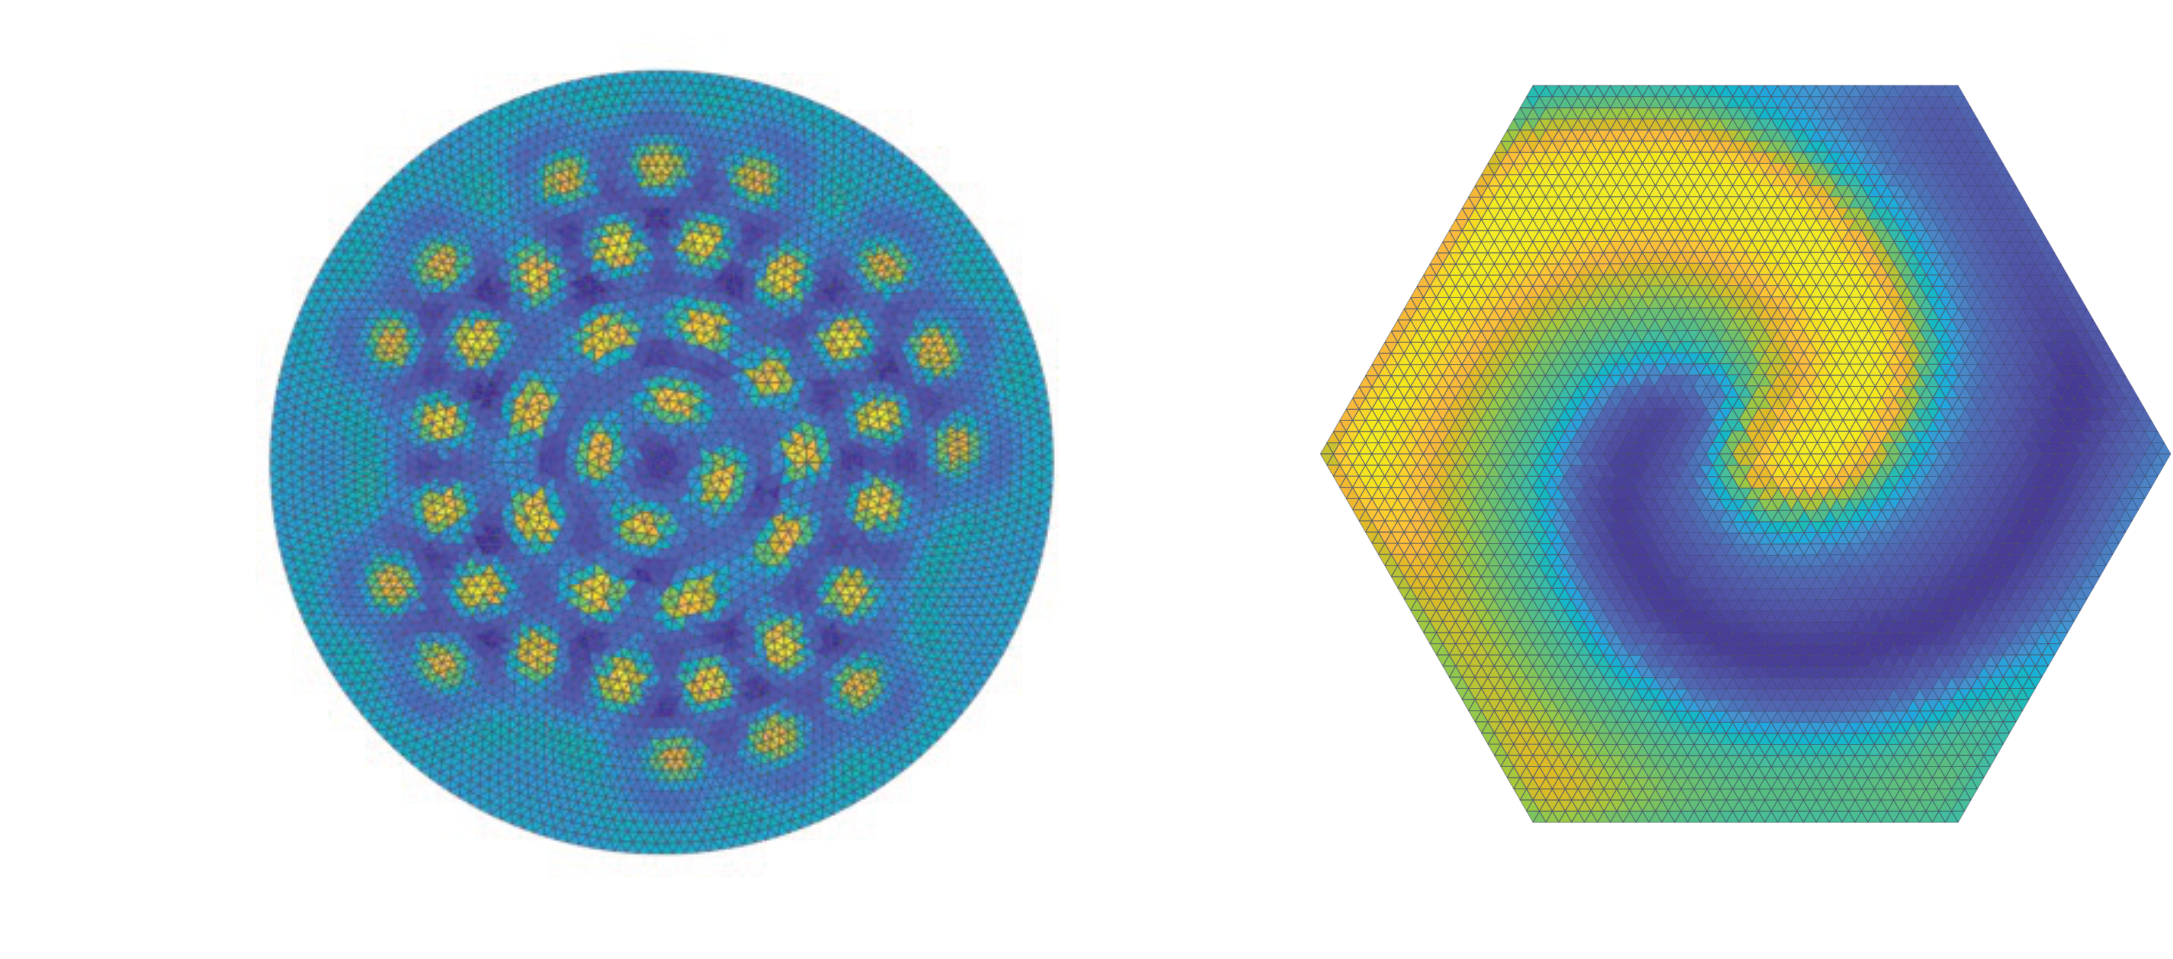
\includegraphics[width = 0.8\textwidth]{patterns}
  \caption{Snapshot of the activity variable $u$ from time simulations of
  \cref{question:spots,question:spiral}.}
  \label{fig:patterns}
\end{figure}
  
\begin{question}\label{question:spiral}
  Cortices support spatiotemporal patterns of activity, and one of the most striking one are rotating waves
  \cite{huangSpiralWavesDisinhibited2004a} (for an experimental recording, download
  \href{https://www.jneurosci.org/highwire/filestream/597325/field_highwire_adjunct_files/4/spiral-s3081907-4500-6775.mpg}{this
  video}). 

  We investigate the formation of spiral waves in neural fields with a \textit{recovery variable}
  $v$ in addition to the activity variable $u$. Simulate the occurrence of spiral
  waves in the model
  % % Right-hand side
  % F = zeros(size(z));
  % F(iU) =  -auu*u - auv*v + b*M*S(u)
  % F(iV) = (-avu*u - avv*v)/tau;
 \begin{equation*}
   \begin{aligned}
     \partial_{t} u(r,t) & = -\alpha u(r,t) -\beta v(r,t) + \nu \int_{D} w(r,r')
     f(u(r',t))\,d r',
       && (r,t) \in D \times [0,T], \\
     \tau \partial_{t} v(r,t) & = -\gamma u(r,t) -\delta v(r,t) 
       && (r,t) \in D \times [0,T], \\
     u(r,0) & = \varphi(r),
       && r \in D, \\
     v(r,0) & = \psi(r),
       && r \in D.
   \end{aligned}
 \end{equation*}

  The cortex $D$ is either the disk of radius $R = 30$ (dataset
  \lstinline|Spiral-Disk|) or a hexagon inscribed in the circle of radius $R=30$
  (dataset \lstinline|Spiral-Hexagon|).

  The synaptic kernel is distance dependent and truncated
  \[
    w(r,r') = W_{A,\eps}(\| r - r' \|_2), 
    \quad 
    W_{A,\eps}(x) = 
    \begin{cases}
      A(x) & \text{if $|A(x)|  \geq \eps $,} \\
      0    & \text{otherwise,} 
    \end{cases},
  \]
  and specified setting $\eps=10^{-3}$ and an integral form for the function $A$,
  involving the Bessel function of the first kind $J_0$
  \[
   A(x) = \int_{0}^{\infty} J_0(xs) \frac{s}{s^4+s^2+1}\,d s.
  \]
  The datasets above provide synaptic and FEM matrices for this kernel on the
  respective grids.

  The firing rate function is given by
  \[
  f(u) = \frac{1}{1+e^{-\mu(u-\theta)}},  \qquad \mu =20, \qquad \theta = 0.6.
  \]
  Note that, in this firing rate, the firing threshold is $\mu \theta$, not $\theta$ as
  in firing rates considered in other questions of the tutorial.

  Observe the formation of spiral waves for $\tau = 5$, $\alpha =1$, $\beta =2$, $\gamma
  =-2.2$, $\delta =1$, $\nu = 3.5$, $T=50$, and initial conditions given by
  \[
    \phi(x,y,z) = 
    \begin{cases}
      1 & \text{if $y > 0$,} \\
      0 & \text{otherwise,} \\
    \end{cases}
    \qquad 
    \psi(x,y,z) = 
    \begin{cases}
      4 & \text{if $x < 0$,} \\
      0 & \text{otherwise.} \\
    \end{cases}
  \]

Once a spiral wave has settled, perturb its core instantaneously, by starting a new
simulation with initial conditions
\[
  \phi(r) = 
  \begin{cases}
    u(r,T) & \text{if $\| r \|_2  > 15$,} \\
    0      & \text{otherwise,} 
  \end{cases}
  \qquad 
  \psi(r) = 
  \begin{cases}
    v(r,T) & \text{if $\| r \|_2  > 15$,} \\
    0      & \text{otherwise,} 
  \end{cases}
\]
and study whether the spiral survives to this large perturbation.
\end{question}

\bibliographystyle{siamplain}
\bibliography{references}

\end{document}
